% !TeX encoding = UTF-8 Unicode
% !TeX root = manual.tex
% !TeX spellcheck = en_GB


\chapter{Examples and expected output}

\section{Example: Searching for s.m.p.-candidates}
This example searches for an s.m.p.-candidate for the set of matrices
$\mathcal{A}=\{A,B\}$.
$A=\tbmatrix{0&0\\1&1}$ and $B=\tbmatrix{1&1\\0&1}$
and shows the expected output.
{\small%
\begin{lstlisting}[style=base]
>> A = [0 0;1 1]; B = [1 1;0 1];
>> c = findsmp( {A,B} );
Search candidate-smp: New bounds: [1.4142135623731, 1.55377397403004]
New bounds: [1.44224957030741, 1.48922284859254]
New bounds: [1.44224957030741, 1.47875763662831]
New bounds: [1.44224957030741, 1.46779926762207]
New bounds: [1.44224957030741, 1.4649600521244]
New bounds: [1.44224957030741, 1.45923280296108]
New bounds: [1.44224957030741, 1.45873105351274]
New bounds: [1.44224957030741, 1.45496833746493]
New bounds: [1.44224957030741, 1.45241564249302]
New bounds: [1.44224957030741, 1.45071633445312]
New bounds: [1.44224957030741, 1.44950376037809]
New bounds: [1.44224957030741, 1.44859499499331]
New bounds: [1.44224957030741, 1.44788857139124]
New bounds: [1.44224957030741, 1.44732368055432]
New bounds: [1.44224957030741, 1.44686166107339]
New bounds: [1.44224957030741, 1.44647675750527]
New bounds: [1.44224957030741, 1.44624360886372]

Bounds on the jsr : [1.44224957030741, 1.44624360886372]
Spectral gap: 1.0004007028302
>> vdisp(c)
(transposed)     1     2     2
\end{lstlisting}%
}


\section{Example: Joint spectral radius of generic matrices}
This example computes the $\JSR$ of the matrices 
$A=\tbmatrix{0&0\\1&1}$ and $B=\tbmatrix{1&1\\0&1}$
and shows the expected output.
{\small%
\begin{lstlisting}[style=base]
>> A = [0 0;1 1]; B = [1 1;0 1];
>> tjsr( {A,B} )
Rough estimate for JSR:    1.000000000000000   1.618033988749895
JSR = [   1.44224957031,   1.61803398875 ], norm=           Inf, #test: 3/3, #V:3/3, 
JSR = [   1.44224957031,             1.5 ], norm= 1.04004191153, #test: 1/1, #V:4/4, 
JSR = [   1.44224957031,   1.44224957031 ], norm=             1, 
Number of vertices of polytope: 4
Products which give lower bounds of JSR: 
(transposed)     1     2     2
@green@Algorithm terminated correctly@
@green@Exact value found.@
JSR =   1.44224957031
\end{lstlisting}%
}

\section{Example: Capacity of code avoiding forbidden differences}
This example computes the capacity of the code with forbidden differences $D=\{\pp\pp\pm\}$
and shows the expected output.
\begin{lstlisting}
>> D = {[1 1 1],[1 1 -1]};
>> C = codecapacity(D)
Base: 2. Generate table of differences. Make bipartite graph adjancy matrix. Compute all locally minimal vertex covers. Generate matrices. 
C = 1×4 cell array
    {4×4 double}    {4×4 double}    {4×4 double}    {4×4 double}
>> r = tjsr( C );
Rough estimate for JSR:    1.618033988749895   2.000000000000000
JSR = [   1.65845707662,               2 ], norm=           Inf, #test: 14/14, #V:6/6, 
JSR = [   1.65845707662,   1.76256137423 ], norm= 1.06277177689, #test: 22/22, #V:16/16, 
JSR = [   1.65845707662,   1.65845707662 ], norm=             1, #test: 16/16, #V:22/22, 
JSR = [   1.65845707662,   1.65845707662 ], norm=             1, 
Number of vertices of polytope: 22
Products which give lower bounds of JSR: 
(transposed)     1     1     3     4     4     2
@green@Algorithm terminated correctly@
@green@Exact value found.@
JSR =   1.65845707662
>> log2(r)
ans =
   0.729841673480343
\end{lstlisting}    

\section{Example: Hölder regularity of Daubechies wavelet}
This example shows how to compute the Hölder regularity of the Daubechies wavelet $D_10$
and shows the expected output.
\begin{lstlisting}
>> T = daubechiesmatrix( 10 )
Computing with vpa. Number of digits: 60
Computing transition matrices.
Computing difference operator.
Condition number for difference operator: 4.35084e+11
Computing transition matrices of difference scheme.
T =
  1×2 cell array
    {10×10 sym}    {10×10 sym}
>> r = tjsr( T );
Rough estimate for JSR:    0.095961983428080   1.413961567654203
Balance 7 Trees. Balancing vector found.
JSR = [ 0.0973017240913,   1.41396156765 ], norm=           Inf, #test: 7/7, #V:10/10, 
JSR = [ 0.0973017240913,  0.364622088673 ], norm= 3.74733430551, #test: 8/8, #V:17/17, 
JSR = [ 0.0973017240913,  0.272489145549 ], norm= 2.80045547079, #test: 16/16, #V:25/25, 
JSR = [ 0.0973017240913,  0.209987621666 ], norm= 2.15810792282, #test: 32/32, #V:41/41, 
JSR = [ 0.0973017240913,  0.161844109947 ], norm=  1.6633221195, #test: 50/50, #V:66/66, 
JSR = [ 0.0973017240913,  0.137391731165 ], norm= 1.41201743801, #test: 50/50, #V:91/91, 
JSR = [ 0.0973017240913,  0.121106808584 ], norm=  1.2446522373, #test: 26/26, #V:104/104, 
JSR = [ 0.0973017240913,  0.116243235454 ], norm= 1.19466778764, #test: 19/19, #V:114/114, 
JSR = [ 0.0973017240913,  0.106835275426 ], norm= 1.09797926423, #test: 14/14, #V:121/121, 
JSR = [ 0.0973017240913,  0.101526835618 ], norm= 1.04342278173, #test: 8/8, #V:125/125, 
JSR = [ 0.0973017240913, 0.0985082310678 ], norm= 1.01239964644, #test: 4/4, #V:127/127, 
JSR = [ 0.0973017240913, 0.0973017240913 ], norm=             1, 
Number of vertices of polytope: 127
Products which give lower bounds of JSR: 
(transposed)     1     1     2     2
@green@Algorithm terminated correctly@
@green@Exact value found.@
JSR = 0.0973017240913
>> -log2( r )
ans =
   3.361390821397782
\end{lstlisting}

\section{Example: Convergence of multiple subdivision scheme}\label{sec_ex_mss}
This example shows how to check the convergence of a multiple subdivision scheme
and shows the expected output.
\begin{lstlisting}
>> S1 = getS( 'a',1/4*[1 3 3 1]', 'M',2, 'n','quadratic bspline' );
>> S2 = getS( '1_4point' );
>> S = [S1;S2]
S =
  2×4 cell array
    {4 sequence}    {[2]}    {1×2 double}    {'quadratic bspline'}
    {7 sequence}    {[2]}    {1×2 double}    {'1_4point'         }
>> blf( S, 'oo',{[1],[1 1 2]} )
ordering: 1 1 1 2 1 1 2 1 1 2 1 1 2 1 1 2 1 1 2 1 1 2 1 1
>> [T,Om] = transitionmatrix( S )
T =
  1×4 cell array
    {6×6 double}    {6×6 double}    {6×6 double}    {6×6 double}
Om =
     0     1     2     3     4     5
>> V = constructVt( Om, 2 )
V =
     1     0     0
    -3     1     0
     3    -3     1
    -1     3    -3
     0    -1     3
     0     0    -1
>> TV = restrictmatrix( T, V )
TV =
  1×4 cell array
    {3×3 double}    {3×3 double}    {3×3 double}    {3×3 double}
>> tjsr( TV );
Rough estimate for JSR:    0.250000000000000   0.295402742514449
Balance 3 Trees. Balancing vector found.
JSR = [            0.25,  0.295402742514 ], norm=           Inf, #test: 2/2, #V:3/3, 
JSR = [            0.25,  0.295402742514 ], norm= 1.70710678119, #test: 1/1, #V:5/5, 
JSR = [            0.25,            0.25 ], norm=             1, 
Number of vertices of polytope: 5
Products which give lower bounds of JSR: 
     1
@green@Algorithm terminated correctly@
@green@Exact value found.@
JSR =            0.25
\end{lstlisting}
\begin{figure}[tb]\centering
    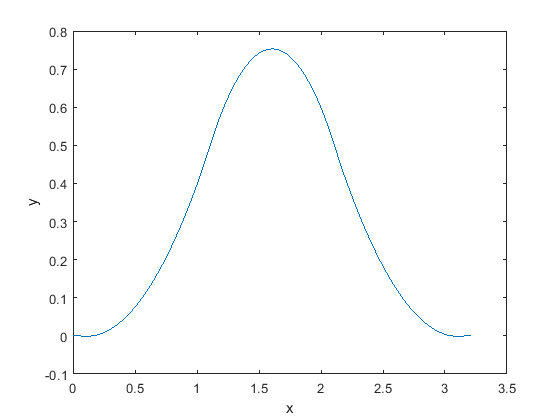
\includegraphics[width=5cm,keepaspectratio]{./graphics/blf}
    \caption{Graphic output of Example~\ref{sec_ex_mss}.}
\end{figure}

%%%%%%%%%%%%%%%%%%%
% EOF
%%%%%%%%%%%%%%%%%%%